\chapter{Justificativa da abordagem}

  \section{Tradicional - RUP}
  Metodologia Tradicional – RUP
            A metodologia tradicional nasceu com o crescimento da computação, onde o nascimento de sistemas empresariais e corporativos necessitou ferramentas para gerenciar grandes projetos. Uma das metodologias tradicionais mais utilizada é o RUP.
            RUP é um framework de processo de engenharia de software que fornece um conjunto de práticas testadas na indústria para desenvolvimento de software e gerência de projetos (Shuja, 2007). Como participante da categoria de metodologia tradicional, o RUP é caracterizado em fases e/ou etapas, e tem um foco alto na documentação do processo.
            Ele é uma metodologia iterativa, na qual basicamente é constituída em quatro fases e diversas iterações entre elas, na qual tem como finalidade tratar questões como planejamento, levantamento e análise de requisitos e entre outros. São elas:
          	\begin{description}
          	\item[$\bullet$] Iniciação: Tarefas de comunicação com o cliente e o planejamento;
          	\item[$\bullet$] Elaboração: Analisar de forma mais detalhada o domínio do problema;
          	\item[$\bullet$] Construção: Construção e desenvolvimento do software;
          	\item[$\bullet$] Transição: Entrega do software e testes.
          	\end{description}
         
 
No RUP também tem as disciplinas, que são basicamente atividades distribuídas ao longo das quatro fases, onde descrevem o que deve ser feito em cada fase com relação à documentação, atividades e outros.
 \begin{figure}[!htpb]
	\centering
	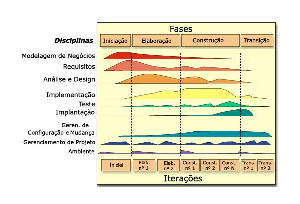
\includegraphics[scale=2.0]{figuras/abordagem/Fases_RUP}
	\caption{RUP}
\end{figure}
As principais características do RUP são:
\begin{description}
		 \item[$\bullet$] Casos de uso: Tem como finalidade capturar os requisitos funcionais do sistema;
         \item[$\bullet$] Centrado na arquitetura: Base do projeto deve ser sólida e estável, mas podendo ser flexível para mudanças e incrementos, ou seja, o sistema deverá ser o mais modularizado possível;
         \item[$\bullet$] Focado no risco: Controla os riscos mais críticos logo no início da fase de Elaboração;
         \item[$\bullet$] Baseado em componentes: Artefatos são construídos a partir da interconexão de objetos projetados através da linguagem UML.
\end{description}
         

